%\documentclass[10pt]{article}
\newcommand{\myGlobalTransformation}[2]
{
    \pgftransformreset;
    \pgftransformcm{1.6}{0}{0.65}{0.5}{\pgfpoint{#1cm}{#2cm}}
}

\newcommand\tru{\hs{T}}
\newcommand\fal{\hs{F}}

\newcommand\ddraw[2]{
        \draw[-,line width=3pt,draw=white] (#1) -- (#2);
        \draw (#1) -- (#2);
}

%\begin{document}
%\pagestyle{empty}

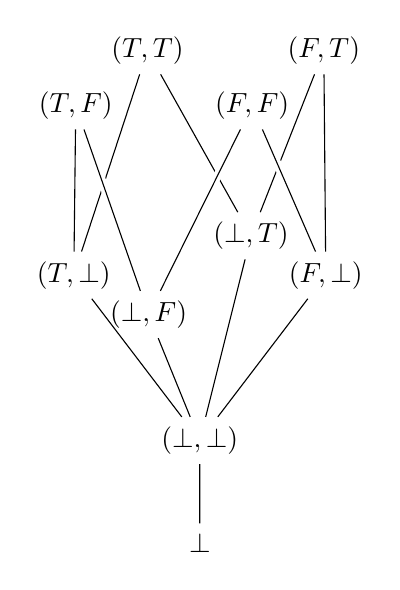
\begin{tikzpicture}

    \begin{scope}
        \myGlobalTransformation{0}{-0.4};
        \node (bottom) at (0,0) {$\bot$};

        \myGlobalTransformation{0}{0.9};
        \node (botbot) at (0,0) {$(\bot,\bot)$};

        \myGlobalTransformation{0}{3};
        \node (trubot) at (-1,0) {$(\tru,\bot)$};
        \node (bottru) at (0,1)  {$(\bot,\tru)$};
        \node (falbot) at (1,0)  {$(\fal,\bot)$};
        \node (botfal) at (0,-1) {$(\bot,\fal)$};

        \myGlobalTransformation{0}{5.5};
        \node (trutru) at (-0.7, 0.7) {$(\tru,\tru)$};
        \node (faltru) at ( 0.7, 0.7) {$(\fal,\tru)$};
        \node (falfal) at ( 0.7,-0.7) {$(\fal,\fal)$};
        \node (trufal) at (-0.7,-0.7) {$(\tru,\fal)$};

        \draw (bottom) -- (botbot);

        \draw (botbot) -- (trubot);
        \draw (botbot) -- (bottru);
        \draw (botbot) -- (falbot);
        \draw (botbot) -- (botfal);

        \ddraw{trubot}{trutru};
        \ddraw{bottru}{trutru};
        \ddraw{falbot}{faltru};
        \ddraw{bottru}{faltru};
        \ddraw{trubot}{trufal};
        \ddraw{botfal}{trufal};
        \ddraw{botfal}{falfal};
        \ddraw{falbot}{falfal};

    \end{scope}

\end{tikzpicture}

%\end{document}